\documentclass[11pt,a4paper]{ltjsarticle} % LuaLaTeX-ja用の日本語対応クラス(A4・11pt)
\usepackage{luatexja} % LuaLaTeXで日本語を扱うための基本パッケージ
\usepackage{luatexja-fontspec} % LuaLaTeXで日本語フォントを指定するための拡張
\usepackage{amsmath,amssymb} % 数式環境・記号の拡張
\usepackage{geometry} % 余白などページレイアウトの調整
\geometry{left=2.5cm,right=2.5cm,top=3cm,bottom=3cm} % ページ余白の具体的な設定
\usepackage{graphicx} % 画像の挿入
\usepackage{booktabs} % 表の罫線を美しくする
\usepackage{siunitx} % SI単位系の表記を統一・自動調整
\sisetup{detect-all,detect-weight=true,detect-family=true} % siunitxの細かい設定(フォント検出など)
\usepackage[
  unicode,bookmarks=true,bookmarksnumbered=true,hypertexnames=false,breaklinks=true,linktocpage=true,
  colorlinks=true,linkcolor=blue,citecolor=blue,urlcolor=blue,pdfborder={0 0 0},pdfpagelabels=false
]{hyperref} % PDFの目次やリンクを有効化・色付け
\usepackage{url} % URLを自動でリンク化
\usepackage{fancyhdr} % ヘッダー・フッターのカスタマイズ
\usepackage{fontspec} % 欧文フォントの指定(LuaLaTeX用)
\usepackage{unicode-math} % 数式フォントの指定(LuaLaTeX用)
\usepackage{pgfplots} % グラフ描画用パッケージ
\pgfplotsset{compat=1.18} % バージョン互換性(必要に応じて調整)
% 欧文フォント設定(例: Times New Roman)
\setmainfont{Times New Roman} % 本文の欧文フォント
\setsansfont{Arial} % 欧文のサンセリフ体
\setmonofont{Consolas} % 欧文の等幅フォント
% 日本語フォント設定
\setmainjfont{Yu Mincho} % 本文の和文明朝体
\setsansjfont{Yu Gothic} % 和文ゴシック体
% 数式フォントもTimes系に統一
\setmathfont{XITS Math} % 数式用フォント(Times系互換)
% 参考文献番号を右肩に上付き表示するためのカスタムコマンド
\newcommand{\supcite}[1]{\textsuperscript{\cite{#1}}} % \citeを上付きで表示


\pagestyle{fancy} % ヘッダー・フッターのカスタムを有効化
\fancyhead{} % 既存のヘッダーをクリア
\fancyhead[R]{\footnotesize
  高周波誘電体材料の革新と応用 \\
  長野高専 電気電子工学科 5年 34番 栁原魁人 \\
  2025年7月10日
} % 右上ヘッダーに情報を表示
% ヘッダー高さ警告の対策
\setlength{\headheight}{34.832pt} % ヘッダー高さを警告値に合わせて調整


\begin{document}
\title{制御工学における安定判別問題}
\author{長野高専 電気電子工学科 5年 XX番 氏名}
\date{2025年7月17日}
\maketitle
\thispagestyle{fancy}

\section{はじめに}
本稿では,高周波領域における誘電体材料の物理的基礎,損失メカニズム,および株式会社TOTOKUのRUOTA技術を中心とした先進的な同軸ケーブル応用について,理論と実践の両面から詳細に分析する.

\section{高周波信号伝送の理論的基礎}
高周波信号伝送では,伝送路材料の物理的挙動が信号品質を大きく左右する.特に誘電体の分極現象,高周波領域でのエネルギー損失,導体の表皮効果が重要である\supcite{ref1,ref2}.

\subsection{誘電体材料と分極の性質}
誘電体は外部電場印加時に内部で分極を生じ,エネルギーを蓄える.分極には電子分極,イオン分極,双極子分極があり,それぞれ応答速度や機構が異なる\supcite{ref2}.分極のしやすさは誘電率($\varepsilon$)で表され,工学的には真空の誘電率$\varepsilon_0$に対する比($\varepsilon_\mathrm{r}$)で議論される.高周波伝送では,低$\varepsilon_\mathrm{r}$材料が信号遅延や減衰抑制の観点から求められる\supcite{ref3}.

\subsection{誘電体におけるエネルギー損失}
高周波交流電場下では,分極の遅れ(誘電緩和)により電場と分極の間に位相差が生じ,エネルギーの一部が熱として散逸する(誘電損失)\supcite{ref1,ref4}.この損失は複素誘電率$\varepsilon^*=\varepsilon'-i\varepsilon''$で表され,$\varepsilon'$は蓄積能力,$\varepsilon''$は損失度合いを示す.損失特性は誘電正接$\tan\delta=\varepsilon''/\varepsilon'$で評価され,$\tan\delta$が小さいほど低損失である\supcite{ref4}.$\varepsilon'$,$\tan\delta$は周波数依存性(誘電分散)を示すため,広帯域で安定した低値が重要である\supcite{ref5}.

\subsection{導体の表皮効果}
高周波電流は導体表面に集中し(表皮効果),有効断面積が減少することで交流抵抗が増大し,導体損失が増加する\supcite{ref1}.表面粗さも損失に影響するため,導体設計も重要である.

\subsection{伝送損失の統一的視点}
伝送損失は主に誘電損失$\alpha_\mathrm{d}$($\propto f\sqrt{\varepsilon_\mathrm{r}}\tan\delta$),導体損失$\alpha_\mathrm{c}$($\propto \sqrt{f}$),散乱損失の和で表される\supcite{ref5}.高周波化に伴い誘電・導体損失が急増するため,材料と構造の最適化が不可欠である.

\section{低損失ケーブルのための材料および構造工学}
\subsection{誘電体材料の選定と製造}
高周波損失低減には,双極子分極の緩和が小さいフッ素樹脂(PTFE,FEP,PFA等)が有効である\supcite{ref14,ref20}.これらは分子構造の対称性により永久双極子モーメントが小さく,$\varepsilon_\mathrm{r}\approx2.1$,$\tan\delta\approx0.0002$と極めて低損失である\supcite{ref14}.押出成形によりケーブル絶縁体として加工される.

\subsection{構造誘電体と中空構造技術}
固体材料の限界を超えるため,空気($\varepsilon_\mathrm{r}\approx1.0$)を構造体に取り込む中空構造が開発された\supcite{ref20,ref22}.TOTOKUのRUOTAはフッ素樹脂絶縁体内部に均一な空気層を設け,実効比誘電率を大幅に低減する.この構造は低損失化,細径化,位相安定性向上など多くの利点をもたらす.


\begin{table}[htbp]
\caption{主要高周波誘電体材料の特性比較(代表値:\SI{10}{\giga\hertz})\supcite{ref5}}
\small % フォントサイズを少し小さくして極端な縮小を回避
\label{tbl:materials}
\centering
\begin{tabular}{lcccp{25mm}} % 特徴カラムを固定幅に
\toprule
材料名 & 比誘電率($\mathit{D}_{\mathrm{k}}$) & 誘電正接($\mathit{D}_{\mathrm{f}}$) & 最高使用温度 & 特徴 \\
\midrule
PTFE & 2.1 & $2.0\times10^{-4}$ & \SI{260}{\celsius} & 最低損失 \\
FEP & 2.1 & $7.0\times10^{-4}$ & \SI{200}{\celsius} & 成形容易 \\
PFA & 2.1 & $5.0\times10^{-4}$ & \SI{260}{\celsius} & 高性能 \\
低損失ポリイミド & 2.6--3.3 & $(2.0$--$2.5)\times10^{-3}$ & \SI{300}{\celsius} & 柔軟 \\
FR-4 & 4.2--4.8 & $(1.5$--$2.5)\times10^{-2}$ & \SI{130}{\celsius} & 一般基板 \\
\bottomrule
\end{tabular}
\end{table}
\normalsize


\section{応用分析:株式会社TOTOKUによる高周波ソリューション}
\subsection{企業・技術プロファイル}
株式会社TOTOKUは「細く,軽く,小さく」を理念に,独自の中空構造技術を核とした高周波・高速伝送ケーブルを展開している.

\subsection{高性能同軸ケーブル「RUOTA」の応用事例}
\subsubsection{5G通信}
RUOTAは5G基地局のMassive MIMOやビームフォーミング用途で,位相安定性・低損失・細径化により高品質通信を支える.

\subsubsection{半導体テスト装置}
THPCシリーズは厳格なインピーダンス管理と細径性で高密度実装・正確な信号伝送を実現する.

\subsubsection{医療機器・産業用途}
TCAシリーズは柔軟・細径・低損失特性により,医療機器や産業機器の高信頼配線に貢献する.

% 特徴の補足:
% TCYCは低損失・細径,THPCは高インピーダンス安定性・厳格な管理,TCAは柔軟・温度位相安定・さらに低損失など,詳細は本文参照。

\section{比較分析と業界動向}
TOTOKUはRUOTA(同軸),Wavemolle(アセンブリ),Leafconn(フラットケーブル)など多様な製品で高周波・高速伝送市場をリードしている.競合他社もフッ素樹脂やFPC等で低損失化を図るが,中空構造技術による差別化が際立つ.

\section{結論}
高周波誘電体材料の進化は,物理学的理解,材料・構造工学,精密製造技術の三位一体で進展している.TOTOKUのRUOTAは中空構造技術により,低損失・細径・高位相安定性を同時に実現し,5G,半導体検査,医療など多分野の基盤技術となっている.

% --- ここから付録データの入れ替え ---

% グラフ描画用パッケージ
% ※プリアンブルに\usepackage{pgfplots}が必要です

\section{付録:オームの法則実験データ}
表\ref{tbl:ohmslaw}に,オームの法則実験のデータを示す.

\begin{table}[htbp]
  \caption{オームの法則実験データ}
  \label{tbl:ohmslaw}
  \centering
  \begin{tabular}{cccc}
    \toprule
    印加電圧[V] & 理論電流[A] & 計測電流[A] & 備考 \\
    \midrule
    0.5 & 0.200 & 0.198 & [ここに備考] \\
    1.0 & 0.400 & 0.400 & [ここに備考] \\
    1.5 & 0.600 & 0.595 & [ここに備考] \\
    2.0 & 0.800 & 0.805 & [ここに備考] \\
    2.5 & 1.000 & 1.010 & [ここに備考] \\
    \bottomrule
  \end{tabular}
\end{table}

\begin{figure}[htbp]
  \centering
  \begin{tikzpicture}
    \begin{axis}[
      width=9cm,
      height=6cm,
      grid=major,
      xlabel={印加電圧 [V]},
      ylabel={電流 [A]},
      legend pos=north west,
      xtick={0.5,1,1.5,2,2.5},
      ytick={0.2,0.4,0.6,0.8,1.0,1.2},
      ymin=0, ymax=1.2,
      xmin=0, xmax=2.7
    ]
    % 計測値(散布図)
    \addplot[
      only marks,
      mark=*,
      color=blue
    ]
    coordinates {
      (0.5,0.198)
      (1.0,0.400)
      (1.5,0.595)
      (2.0,0.805)
      (2.5,1.010)
    };
    \addlegendentry{計測電流}
    % 理論値(直線)
    \addplot[
      domain=0:2.5,
      samples=100,
      color=red
    ]{0.4*x};
    \addlegendentry{理論電流}
    \end{axis}
  \end{tikzpicture}
  \caption{オームの法則実験データのグラフ}
  \label{fig:ohmslaw}
\end{figure}

% --- ここまで付録データの入れ替え ---

% --- 付録:サイクロイドのグラフ ---
\begin{figure}[htbp]
  \centering
  \begin{tikzpicture}
    \begin{axis}[
      width=12cm,
      height=6cm,
      grid=major,
      xlabel={$x$},
      ylabel={$y$},
      axis equal,
      xmin=0, xmax=12.57,
      ymin=0, ymax=2.5,
      xtick={0,3.14159,6.28318,9.42477,12.5664},
      xticklabels={0,$\pi$,$2\pi$,$3\pi$,$4\pi$},
      title={サイクロイド曲線(半径 $r=1$)}
    ]
    % サイクロイド曲線
    \addplot[
      domain=0:4*pi,
      samples=200,
      thick,
      blue
    ]
    ({x - sin(deg(x))}, {1 - cos(deg(x))});
    \end{axis}
  \end{tikzpicture}
  \caption{サイクロイド曲線 $x = r(t - \sin t)$,$y = r(1 - \cos t)$}
  \label{fig:cycloid}
\end{figure}

% --- 付録:サインとコサインのグラフ ---
\begin{figure}[htbp]
  \centering
  \begin{tikzpicture}
    \begin{axis}[
      width=12cm,
      height=6cm,
      grid=major,
      xlabel={角度 $\theta$ [rad]},
      ylabel={振幅},
      legend pos=north east,
      xmin=0, xmax=12.57,
      ymin=-1.2, ymax=1.2,
      xtick={0,1.5708,3.14159,4.71239,6.28318,7.85398,9.42477,10.996,12.5664},
      xticklabels={0,$\frac{\pi}{2}$,$\pi$,$\frac{3\pi}{2}$,$2\pi$,$\frac{5\pi}{2}$,$3\pi$,$\frac{7\pi}{2}$,$4\pi$},
      title={正弦波と余弦波}
    ]
    % sin関数
    \addplot[
      domain=0:4*pi,
      samples=200,
      thick,
      red
    ]{sin(deg(x))};
    \addlegendentry{$\sin \theta$}
    % cos関数
    \addplot[
      domain=0:4*pi,
      samples=200,
      thick,
      blue
    ]{cos(deg(x))};
    \addlegendentry{$\cos \theta$}
    \end{axis}
  \end{tikzpicture}
  \caption{正弦関数と余弦関数の周期特性}
  \label{fig:sincos}
\end{figure}

% --- 付録:回路図イメージの挿入 ---
\begin{figure}[htbp]
  \centering
  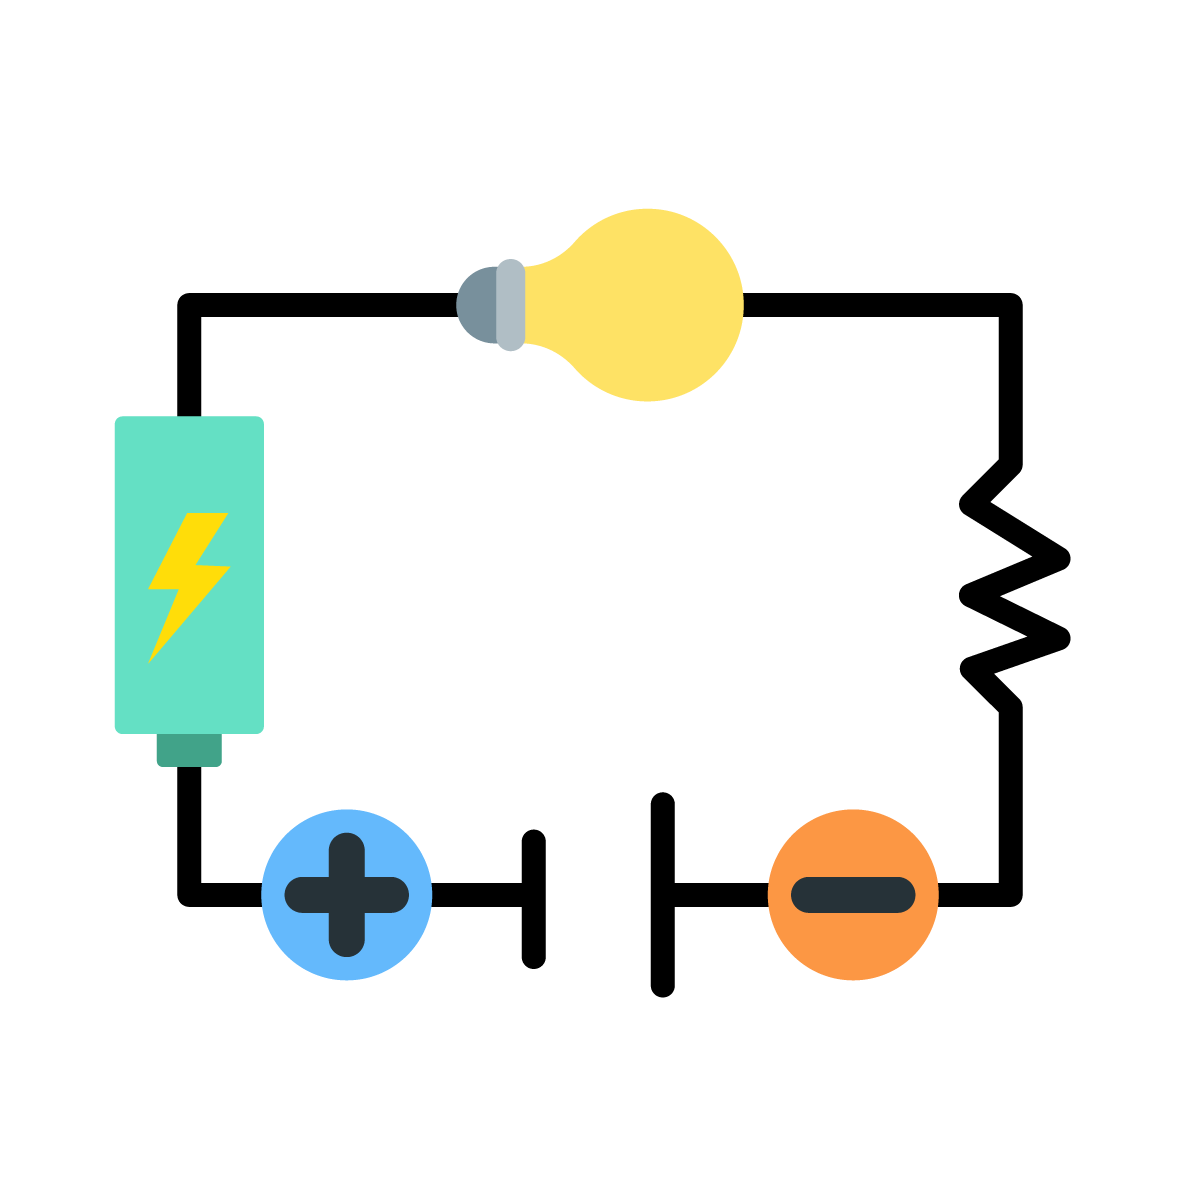
\includegraphics[width=0.6\linewidth]{—Pngtree—electrical circuit_8178136.png}
  \caption{電気回路のイメージ(出典:Pngtree)}
  \label{fig:circuit_image}
\end{figure}
% --- 付録ここまで ---

\begin{thebibliography}{99}
\bibitem{ref1} 精電舎電子工業「高周波誘電加熱とは」\url{https://www.sedeco.co.jp/technology/list/hfw/}
\bibitem{ref2} 東亞合成「高分子の誘電特性」\url{https://www.toagosei.co.jp/develop/item/no21_02.pdf}
\bibitem{ref3} 東京工業大学「ポリイミドの6G周波数域における誘電特性を解明」\url{https://www.titech.ac.jp/news/2024/069742}
\bibitem{ref4} crowdchem.net「誘電正接とは?」\url{https://crowdchem.net/column/985/}
\bibitem{ref5} Resonac「伝送損失・誘電損失・誘電正接とは?」\url{https://www.resonac.com/jp/solution/tech/transmission-loss.html}
\bibitem{ref14} 株式会社TOTOKU「高周波ケーブルとは?」\url{https://www.totoku.co.jp/special-contents/column/coaxial_13/}
\bibitem{ref20} TOTOKU「RUOTA Equipment Lead Cable」\url{https://en.totoku.co.jp/product/coaxial-lead/}
\bibitem{ref21} Shibata Co., Ltd.「High Performance Coaxial Cable (RUOTA)」\url{https://www.shibata.co.jp/english/products/ruota}
\bibitem{ref22} TOTOKU「High performance Coaxial Cable」\url{https://www.totoku.co.jp/wp/wp-content/themes/totoku/assets/doc/en-RUOTA.pdf}
\end{thebibliography}

\end{document}
